\documentclass[12pt,letterpaper,twoside]{article}
\usepackage{cme211}

\usepackage{atbegshi}% http://ctan.org/pkg/atbegshi
\AtBeginDocument{\AtBeginShipoutNext{\AtBeginShipoutDiscard}}

\begin{document}
\title{Lecture 5: Objects, Modules, and Exceptions\vspace{-5ex}}
\date{October 9th, 2018}
\maketitle

{\footnotesize
\paragraph{Topics Introduced:} Python object model, 
modules, and exceptions.
}
\vspace{-3ex}
\section{Python Object Model}
Let's review and elaborate on Python's object model. Key things to
always keep in mind:

\vspace{-2ex}
\begin{enumerate}
\item
  Everything in Python is an \textbf{object}.

  An object is a location in memory associated with both a type and a value.
\item
  Variables in Python are \textbf{references} to objects.
\end{itemize}

\vspace{-3ex}
\paragraph{Simple List Example} What happens when we create a list, 
and then assign another variable to the same data?

\begin{python}
a = [42, 19, 73]
b = a
\end{python}

We would hope that the variable \texttt{b} should be ``the same'' as \texttt{a}, 
in the sense that we expect them to be element-wise equal. But is the underlying
data in fact the same? I.e. are we referencing the same object in memory? 

\begin{python}
b[0] = 7   # This assignment modifies first element ref'd by var 'b'.
print(b)   # This mutates data pointed to not only by 'b' ...
print(a)   # ... but also the data pointed to by variable 'a'.
\end{python}

\begin{figure}[!h]
\centering
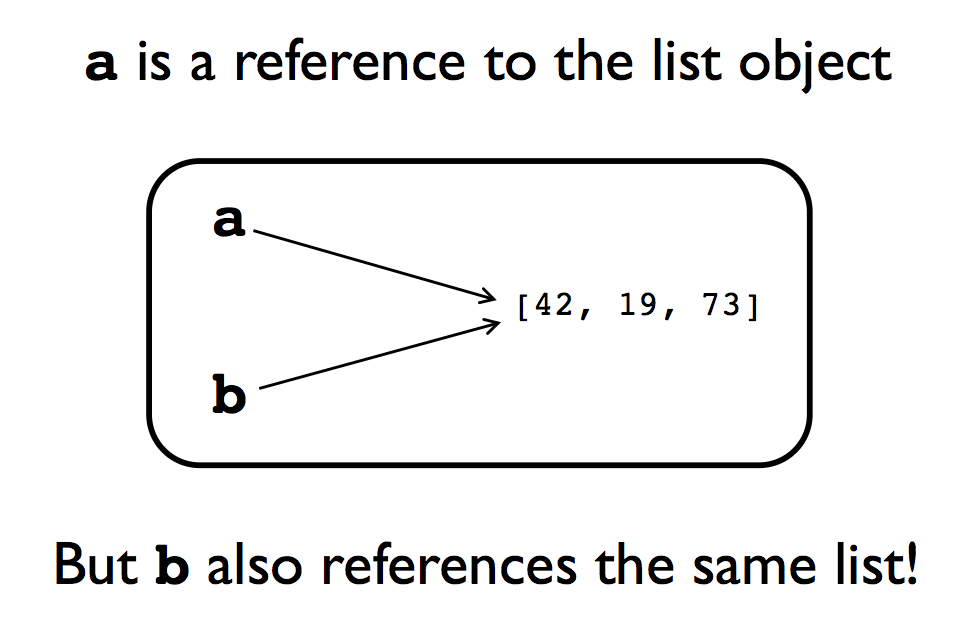
\includegraphics[scale=0.35]{fig/references.png}
\caption{{ \small Variables in Python are \emph{references} to objects.}}
\end{figure}

In this example, \texttt{a} is a reference to the list object initially
set to \texttt{{[}42,\ 19,\ 73{]}}. The variable \texttt{b} also
references the same list.

\paragraph{References: Analogies}   This room is like an object.
\begin{itemize}
\item
  ``Hewlett Auditorium (ii)'' is an identifier that references this room.
\item
  ``Hewlett-201'' is also an identifier that references this same room.
\end{itemize}

Or perhaps more familiar, we assign identifiers to family members based on their relation
to ourselves. E.g. when I say ``my sister'', I am referring to 
\href{https://soundcloud.com/monikasantucci}{Monika Santucci}.

We emphasize that different identifiers can refer to the same data.

\vspace{-3ex}
\subsection{Python is Dynamically and Strongly Typed}
Python is a 
\href{https://en.wikipedia.org/wiki/Type_system#Dynamic_type_checking_and_runtime_type_information}{dynamically typed} 
language, which is in contrast to a 
\href{https://en.wikipedia.org/wiki/Type_system#Static_type_checking}{statically typed} language such as C++. 
Note that both are still considered \emph{typed} languages.\footnote{In an untyped language, neither identifiers
nor the data which they point to are associated with a type. E.g. the programming language \href{https://en.wikipedia.org/wiki/B_(programming_language)#History}{B} is untyped: every variable refers to a \href{https://en.wikipedia.org/wiki/Word_(computer_architecture)}{\emph{word}} of memory. Depending on the \emph{context}
in which the variables appear, the data will be treated differently, either as an integer value, a string, or a pointer which is to be dereferenced.}

\paragraph{Statically Typed} languages attempt to resolve errors and find potential bugs at \emph{compile time}.
If the compiler knows exactly the type of each variable, then the generated machine code can be optimized, resulting in code which potentially executes faster
at run time. 

\paragraph{Dynamically Typed} languages, on the other hand, 
will delay inspecting the underlying data types that appear in an expression until \emph{run time}. Note that this means that when source code is modified,
the interpreter is permitted to dynamically load new code without checking for fool-proof compatibility with all other parts of the program.

Identifiers in Python are dynamic, and aren't necessarily tied to a single type of data.

E.g. an identifier can reference an
integer at one point in time, and then later a string.

\begin{python}
a = 5
a = 'hi'
\end{python}

\vspace{-3ex}
\paragraph{Strongly Typed} Python is also
\href{https://en.wikipedia.org/wiki/Strong_and_weak_typing#Definitions_of_%22strong%22_or_%22weak%22}{\textbf{strongly typed}}.
The Python interpreter will inspect types at runtime, as they are being
executed (since it is dynamically typed), \emph{but} certain classes or errors are precluded from happening (since it is strongly typed):
implicit conversions between disparate types is disallowed.
  
E.g. you can't add a number and a string in base Python, because the language rules state that operation doesn't make sense.\footnote{This is in contrast to a weakly typed language, such as Perl, wherein the type of one object may be coerced to match another type such that an operation may be carried out. E.g. if you try to use operator \texttt{+} on an integer and a string, Perl will coerce the string to an integer (using the additive identity 0) and then perform the addition.}

\subsection{Assignment: Setting Up a Reference}
\vspace{-1ex}
We restate that everything in Python is an object: numbers, strings, functions, etc. are all objects;
an object is simply a location in memory associated with a type and a value.
The assignment operation, \texttt{=}, can be interpreted as setting up a
reference. E.g.

\begin{python}
a = 'hello'
\end{python}

We may pedagogically interpret this as a two part operation.
\vspace{-2ex}
\begin{enumerate}
\item
  Create a string object containing
  \texttt{\textquotesingle{}hello\textquotesingle{}}.
\item
  Set up the identifier \texttt{a} to refer to the newly created string
  object.
\end{enumerate}

Illustrations and more examples may help.
\vspace{-1ex}
\begin{figure}[h]
\centering
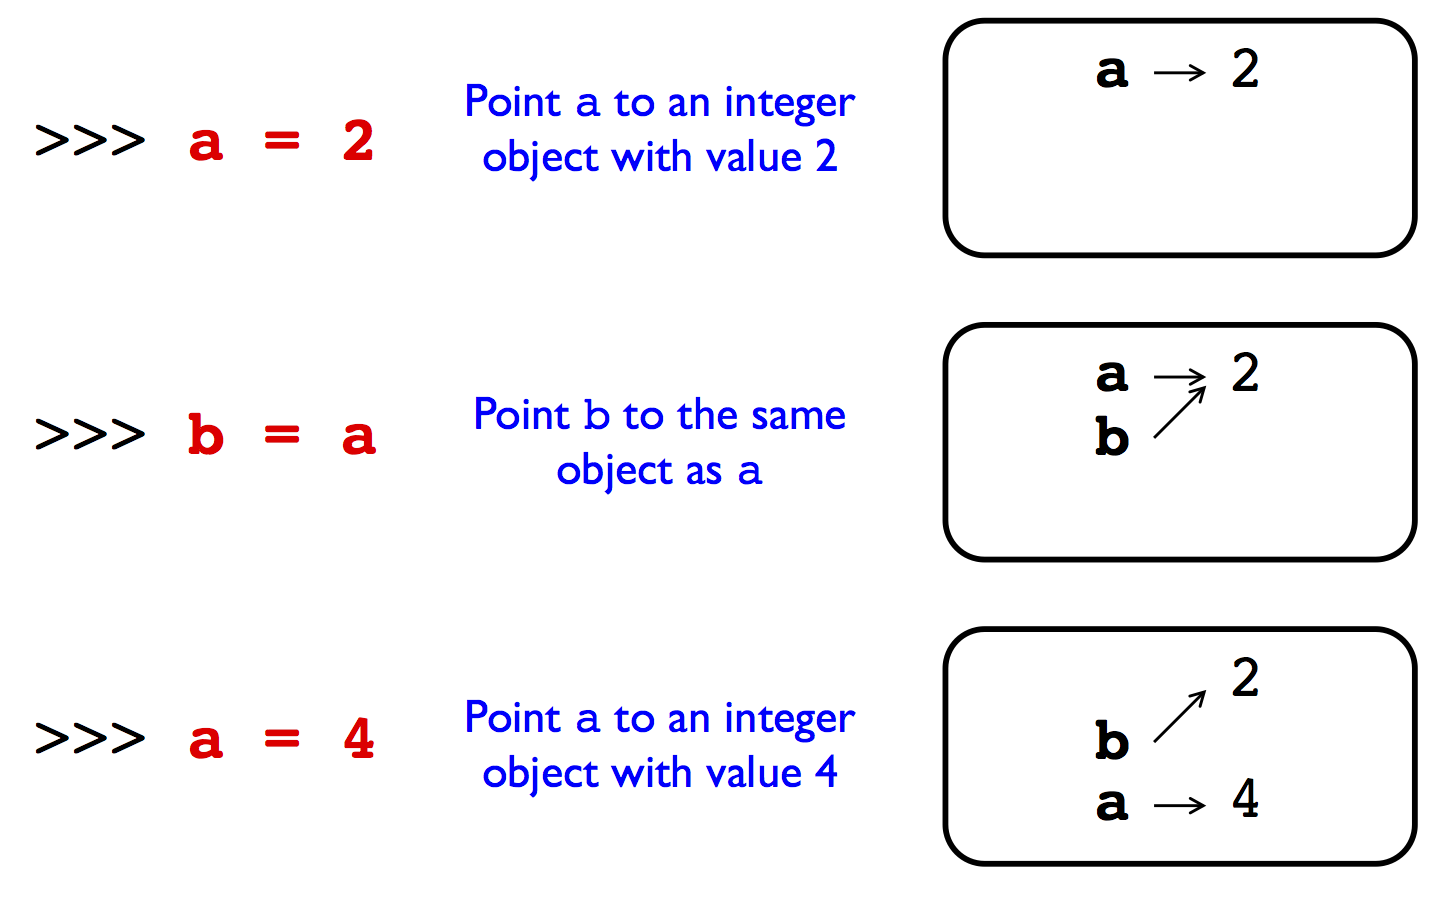
\includegraphics[scale=0.35]{fig/references-example.png}
\caption{\small An object is a location in memory with a type and value. The boxed region can be interpreted as a memory layout or diagram.
The location in the diagram which a value appears corresponds to the location in memory in which the object is stored. Here, we leave types implicit.}
\end{figure}

% We remark that we even must (implicitly) create temporary objects for intermediary values used in expressions.

\begin{figure}[h]
\centering
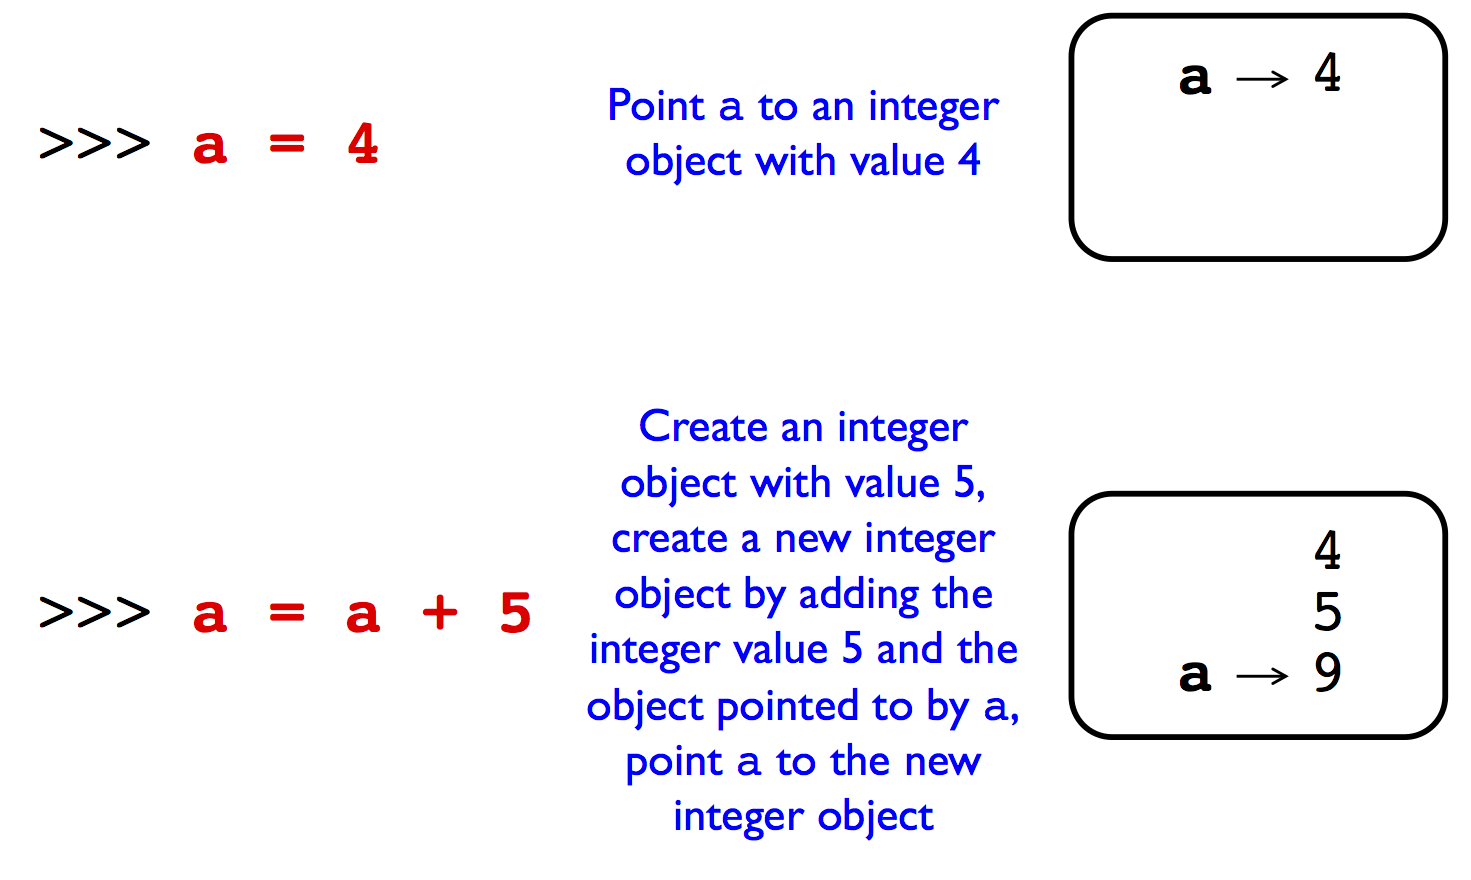
\includegraphics[scale=0.35]{fig/references-example-2.png}
\caption{\small Integers are also objects and must be created in memory. E.g. in order to ``add 5'' to an object, 
we first have to define a reference to the integer value 5, then use this data as part of an input to an \texttt{add} operation.}
\end{figure}

\subsection{References (Details)}
\subsubsection{Checking References}
We can check if two names (variables) reference the same object with the
\href{https://docs.python.org/3/library/operator.html}{\texttt{is}} operator.\footnote{
Implementation detail in CPython: 
the \href{https://docs.python.org/3/library/functions.html#id}{\texttt{id}} operator 
returns the position in memory where the object is stored.
}

\begin{python}
a = [42, 19, 73]
b = a
print(a is b)
\end{python}

In memory we may visualize the following schematic.

\begin{figure}[h]
\centering
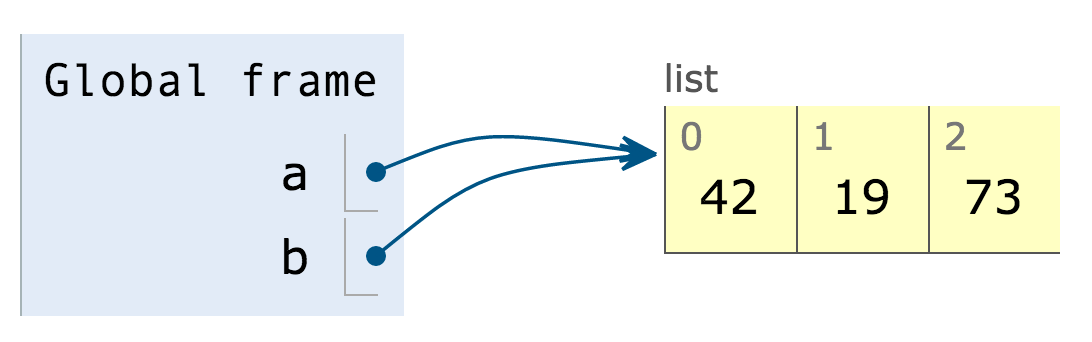
\includegraphics[scale=0.5]{fig/list-1.png}
\caption{The \href{https://docs.python.org/3/library/operator.html}{\texttt{is}} operator checks to see if two references point to the same object. I.e. it can be seen as a test of \emph{identity}.}
\end{figure}

\begin{python}
b = [42, 19, 73]
print(a is b)
\end{python}

In memory we have:

\begin{figure}[h]
\centering
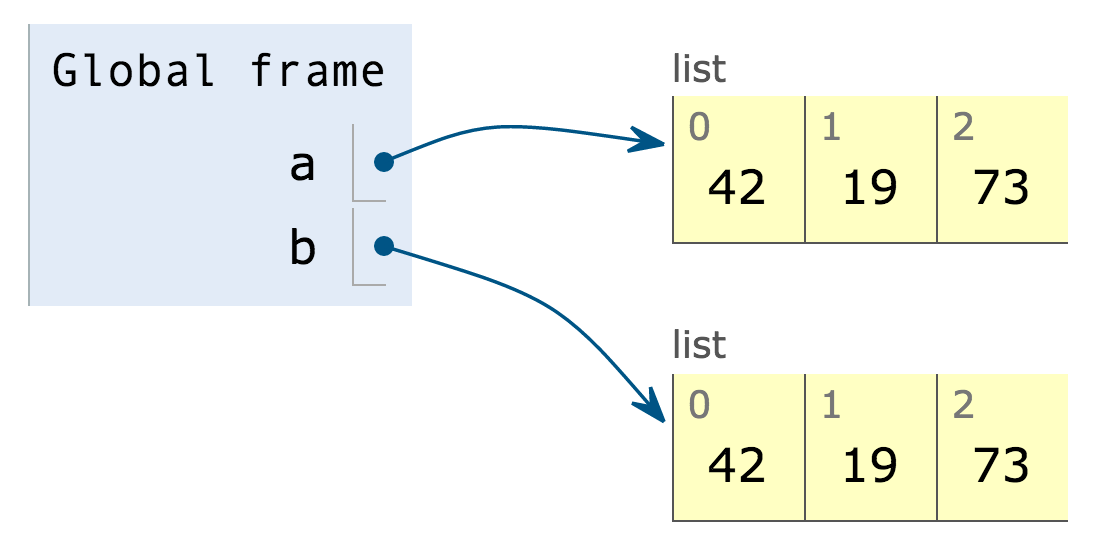
\includegraphics[scale=0.35]{fig/list-2.png}
\caption{If we assign \texttt{b = [42, 19, 73]}, then even though the values are the same, we can really think of the data as being different. Mutating one object will not affect the other.}
\end{figure}

Check it out in
\href{http://www.pythontutor.com/visualize.html\#code=a\%20\%3D\%20\%5B42,\%2019,\%2073\%5D\%0Ab\%20\%3D\%20a\%0Aprint(a\%20is\%20b\%29\%0Ab\%20\%3D\%20\%5B42,\%2019,\%2073\%5D\%0Aprint(a\%20is\%20b\%29\%0A\&cumulative=false\&curInstr=0\&heapPrimitives=false\&mode=display\&origin=opt-frontend.js\&py=3\&rawInputLstJSON=\%5B\%5D\&textReferences=false}{Python Tutor}.
There's one more nuance to this diagram that we need to refine, and that is how small (magnitude) integers are stored permanently.

\subsubsection{Integers and References}
Integers are objects also and need to be created in memory. Let's
explore this a bit.

\begin{python}
a = 1024
b = a
a is b     # Returns True: we asked 'b' to refer to same data as 'a'.
\end{python}

\begin{python}
a = 1024   
b = 1024   # Python creates a *new* integer (diff location), also with value 1024.
a is b     # Returns False: 'a' and 'b' refer to different pieces of data.

a = 16
b = 16
a is b     # For small integers, Python reserves persistent storage.
\end{python}

In the last code block, \texttt{a} and \texttt{b} point to the same
object, because Python preallocates some integers. This is done as an 
\href{https://docs.python.org/3/c-api/long.html}{internal optimization for the Python interpreter written in C}.

\vspace{-2ex}
\paragraph{Preallocated Integers (an Implementation Detail)}
Python creates permanent storage for integer objects in the range $\{-5, ..., 256\}$, instead of 
constantly creating and destroying these objects which we anticipate to be frequently used.
Integers outside this range are created and destroyed on an as-needed basis.

\begin{python}
a = -6   # Here, we create two separate integer objects...
b = -6   # ... in memory. Different locations, but same values.
a is b   # Returns False.

a = -5   # The C-API has written an optimization such that we...
b = -5   # ... don't constantly create/destroy integers in [-5, 256].
a is b   # Returns True accordingly.

a = 256
b = 256
a is b   # Returns True, since [-5, 256] all stored permanently.

a = 257  # Here, we're outside the range of [-5, 256].
b = 257  # Whence this is a different object in memory.
a is b   # Returns False.
\end{python}

Of course, this is all very different from the \href{https://docs.python.org/3.4/library/operator.html#operator.eq}{\texttt{operator.eq}}, i.e. \texttt{==}.

\vspace{-3ex}
\subsubsection{String Reuse (Another Implementation Detail)}
\begin{python}
a = 'hello'
b = 'hello'
a is b      # Returns True. For a longer arbitrary string, may return false.
\end{python}

\vspace{-2ex}
\paragraph{Why are Strings Immutable?}
Let's consider why we might preference strings to be immutable.\footnote{This is totally separate from ``reusing'' an object, i.e. wherein two identifiers refer
to the same data.} An \textbf{immutable} object can't be modified. The reasons relate to \emph{performance}.\footnote{We remark that this is a design decision not uncommon in other languages (e.g. Java strings).}
\begin{itemize}
\item Can setup storage for a string exactly once, because it never changes.
\item Dictionary keys required to be immutable, so that we can quickly locate keys.
\end{itemize}

\subsection{Containers and Element References}
It's important to realize that Collections store other data (structures), i.e. an element of a data structure
is simply an object (a location in memory associated with a value and a type).

\begin{itemize}
\item
  Elements in a list, or key and value pairs in a dictionary,
  contain references to objects.
\item
  Those references can be to ``atomic'' data types like a Boolean, number, or
  string. They can also be to more complicated data types, like other containers.
\item
  There are some restrictions, for example we've discussed that the key objects in a
  dictionary must be immutable (e.g. numbers, strings, or tuples).
\end{itemize}

\vspace{-3ex}
\begin{python}
a = [42, 'hello']
b = a
\end{python}
\vspace{-2ex}
\begin{figure}[h]
\centering
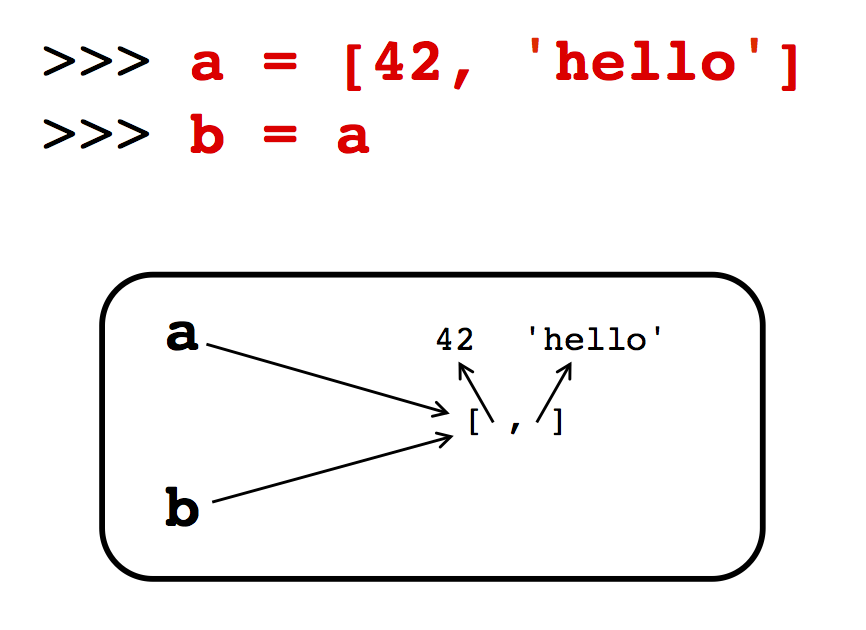
\includegraphics[scale=0.35]{fig/list-ref.png}
\caption{\small A more accurate memory diagram reveals that individual elements of an Abstract Data Type are simply
references to other objects, which themselves can be atomic or another ADT.}
\end{figure}

\vspace{-3ex}
\subsection{Copying: Shallow vs. Deep Copy}
We must emphasize that simple assignment does not give us a copy of the object (e.g. a list), only an
additional reference to the same object (list in our example). It's natural to ask: 
what if we really want an additional copy that can be modified without
changing the original?

\paragraph{Shallow copy}
A shallow copy (\texttt{copy.copy}) constructs a new list and inserts
references to the objects referenced in the original.

\begin{python}
a = [42, 'hello']
import copy
b = copy.copy(a)
\end{python}

\begin{figure}[h]
\centering
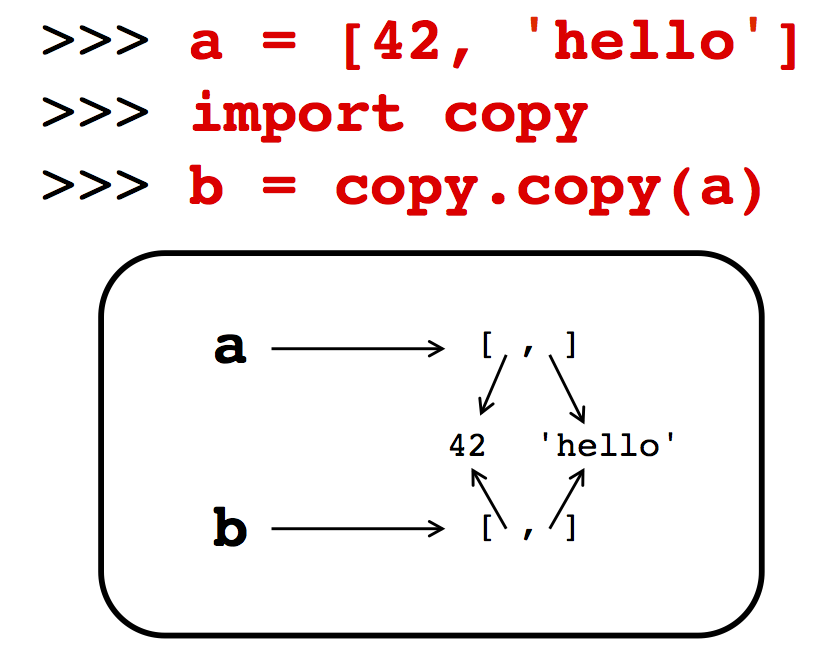
\includegraphics[scale=0.35]{fig/shallow-copy.png}
\caption{\small A shallow copy creates a \emph{new list}, where each element refers to the same
  element referred to by the original list entry.}
\end{figure}

\paragraph{Shallow Copies and Mutables} Note that since a shallow copy simply sets up references
to the same underlying objects, then if said objects are mutable we can inadvertently run into
results that at first surprise us.
\begin{python}
a = [19, {'grade':92}]
b = copy.copy(a)

a[0] = 42             # Modifies first element of 'a' only.
print(b)              # First element of 'b' still refers to integer 19.
a[1]['grade'] = 97    # Here, we modify the dictionary referred to by both 'a' and 'b'.
print(b)              # Accessing 'b["grade"]' returns integer value 97.
\end{python}

\begin{figure}[h]
\centering
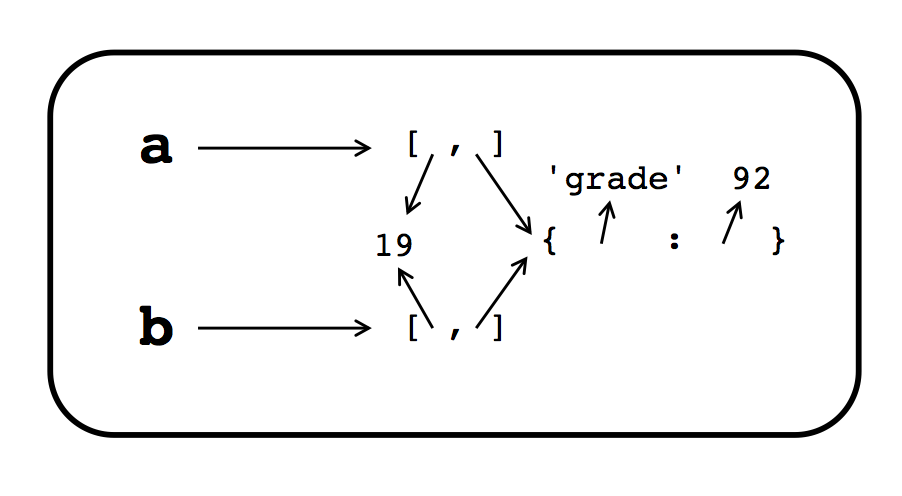
\includegraphics[scale=0.35]{fig/shallow-copy-mutables.png}
\caption{A shallow copy sets up references to the same underlying data of the original container. Since object \texttt{a} contains a dictionary,
then upon shallow copy to variable \texttt{b}, the first element in either variable in fact refers to the same dictionary.}
\end{figure}

This may not be desireable in all cases, whence there is also a \emph{deep copy} sub-routine.

\paragraph{Deep Copy} A deep copy (\texttt{copy.deepcopy}) constructs a new list and inserts
copies of the objects referenced in the original. It will (recursively) copy all
nested data structures. 

\begin{python}
a = [19, {'grade':92}]
b = copy.deepcopy(a)

a[0] = 42           # Request first element of 'a' to refer to integer 42.
a[1]['grade'] = 97  # Request the dictionary ref'ed by 'a' to update value associated with 'grade'. 
\end{python}

\begin{figure}[h]
\centering
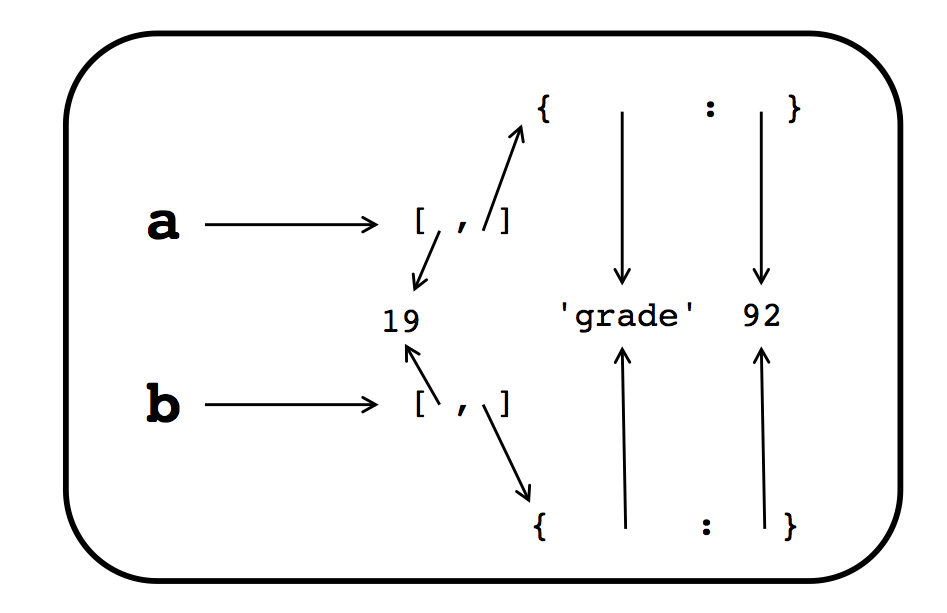
\includegraphics[scale=0.35]{fig/deep-copy-mutables.png}
\caption{\small In a \emph{deep copy}, each element is a copy of the object referenced by the corresponding
  element in the original container. Since strings may be re-used, and since we are only dealing with
  integers in the set $\{-5, \ldots, 256\}$, datum are not duplicated (i.e. the implementation details
  don't require there to be additional copies of the string \texttt{grade} or the integers 19, 92.}
\end{figure}

\subsection{Tuples and Immutability}
Let us revisit the nuances relating to tuples and immutability: the length of the tuple and which objects
are referred to by the tuple are fixed from the time of creation.

\begin{python}
a = [42, 'feed the dog', 'clean house']
import copy
b = copy.copy(a)  # Set up references to same underlying objects.
c = (a,b)         # Create a tuple. Since 42 in {-5, ..., 256} and strings may ...
                  # ... be re-used, then even though the lists are different...
                  # ... the underlying data referrenced is the same.

b[0] = 7          # Here, we ask the first element of 'b' to refer to integer 7.
print(c)          # Of course, first element of 'a' still references integer 42.
c[0][0] = 7       # We can change the first element of 'a' as well...
print(c)          # ... and this will be reflected here.

# c[0] = [73, 'wash dishes', 'do laundry'] --> Error: Tuple object disallows item assignment.
\end{python}

\begin{figure}[h]
\centering
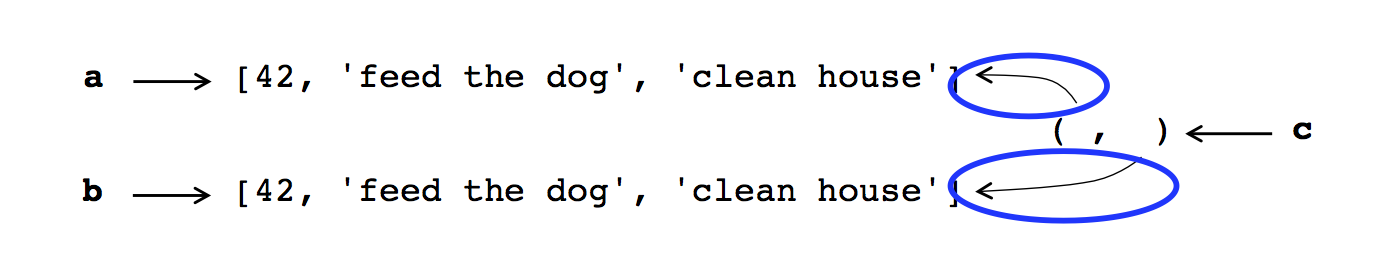
\includegraphics[scale=0.45]{fig/tuples-and-immutability.png}
\caption{In this memory diagram, the integers and strings need not be duplicated 
(since the integers appearing are in the set $\{-5, \ldots, 256\}$ and strings may
be reused). However, the important part is that while we can never change the fact that 
\texttt{c} is a tuple of length two, where each element is a list, we can modify the underlying
lists themselves. E.g. aside from the example pictured, we could also query 
\texttt{[c[0].pop() for i in range(3)]} in order to leave the object referenced by variable 
\texttt{a} an empty list.}
\end{figure}

The immutable property of tuples only means I can't add or remove elements from the tuple, and I can't
ask the elements of the tuples to refer to different objects. However, the underlying objects themselves
can be changed if they are mutable.

\subsection{Memory Management}
What happens to objects that are no longer referenced?

\begin{figure}[h]
\centering
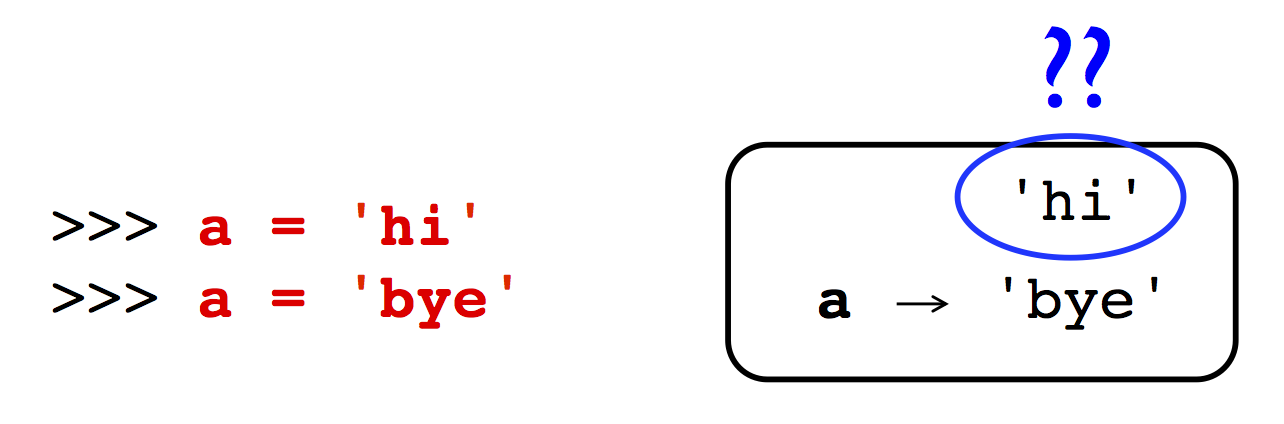
\includegraphics[scale=0.35]{fig/gc-1.png}
\caption{Motivating Garbage Collection: Unlike the integers $\{-5, \ldots, 256\}$, strings aren't guaranteed
to persist in a single location in memory, even though both types are immutable. What happens to strings (or any object) when we
``don't need them anymore''?}
\end{figure}

\paragraph{Garbage Collection}
When an object is no longer reachable or accessible via an identifier, it may be \href{https://en.wikipedia.org/wiki/Garbage_collection_(computer_science)}{garbage collected};
the idea is simple: if an object requires resources but is no longer being used, we may as well free said resources for other parts of our program (or operating system) to use. 
Python implements garbage collection via \href{https://en.wikipedia.org/wiki/Reference_counting#Use_in_garbage_collection}{reference counting}.

\begin{figure}[h]
\centering
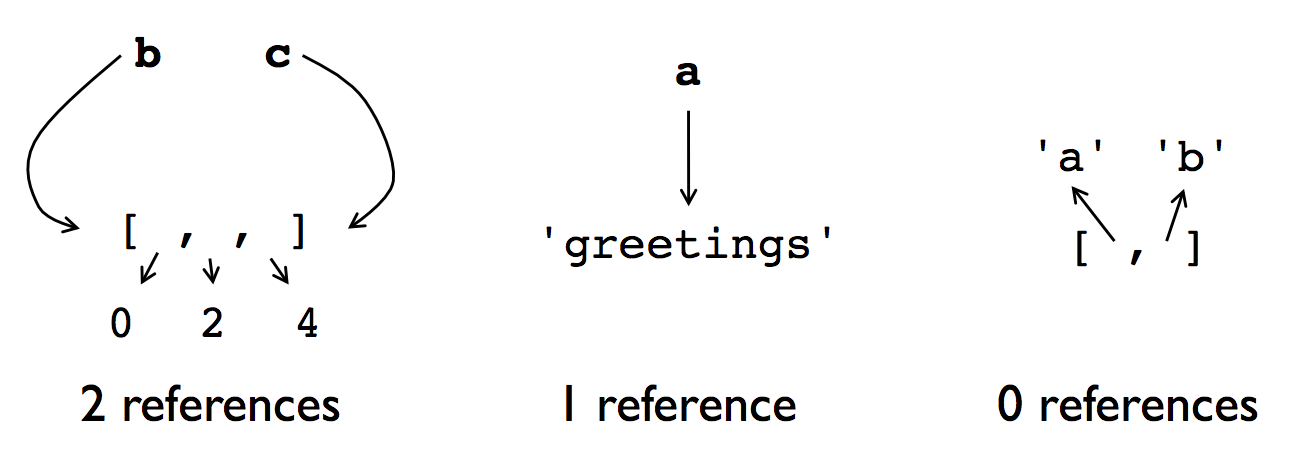
\includegraphics[scale=0.35]{fig/gc-2.png}
\caption{The first example on the left depicts a case where each integer is referenced by two variables, i.e. 
lists \texttt{b} and \texttt{c} (which in this example happen to refer to the same list). In the second example in the middle, we depict
a case where a string ``greetings'' is referenced by a single variable \texttt{a}. In the last example on the right, we have a single 
unreferenced list, where the elements themselves are ``a'' and ``b''. However, since the list is not aliased to any variable, these 
character elements are inaccessible. Even though strings are immutable, Python doesn't require we store them throughout the program's entirety.
Whence we may garbage collect these data (each of the characters, and in fact the list as well).}
\end{figure}

\subsection{Recommended Reading}
Chapter 6: The Dynamic Typing Interlude, from ``Learning Python'', by Klutz.

%%%%%%%%%%%%%%%%%%%%%%%%%%%%%%%%%%%%%%%%%%%%%%%%%%

\section{Python Modules}

\subsection{Modules as an Organizational Tool} Your code should be organized in some way.
We often split code across multiple files to make it easier to maintain and re-use.

For larger projects, we in fact often have multiple directories, each with multiple files.

E.g. consider the grading tools we might use for CME211. We might have a set of sub-routines that lets
us fetch student repositories from Github and later push feedback, and it would make sense for this code
to set in its own file. On the other hand, we also might have a set of sub-routines that actually
perform integration tests on your programs. This grading utility tools have nothing to do with our Git utils, and so we place it
in another file as well. But! All the code is useful for this class as a whole, and so we place it within a \texttt{CME211} module.

\subsection{Using Modules - Practical Details} Code in Python is organized and accessed via \emph{modules}. We've already seen and used  examples such as
\texttt{math} and \texttt{time}; they are accessed using an \texttt{import} statement.

\subsubsection{Basic Usage}
\paragraph{Import}
Here is an example of importing and using a function from the
\texttt{time} module:

\begin{python}
import time
time.time()    # Prints out current time in seconds since the Epoch (Jan 1st, 1970)

# time()                --> Error: time module is not callable.

print(type(time))       # <class 'module'>
print(type(time.time))  # <class 'builtin_function_or_method'>

\end{python}
We must keep in mind that the module name/object is different 
than the function that exists inside of the module.

\paragraph{Reference to a Function}
Functions are also objects and may be assigned to a variable:

\begin{python}
t = time.time
type(t)          # <builtin_function_or_method>
t is time.time   # True.
t()              # Returns time in seconds since Epoch.
\end{python}

Everything in Python is an object!

\paragraph{Importing a Single Function}
We can import a single function from a module:

\begin{python}
from time import time
print(type(time))   # <class 'builtin_function_or_method'>
print(time())       # Returns time in seconds since Epoch.
\end{python}

Here, we've created an alias for the \texttt{time.time()} sub-routine. 
Another example is \texttt{from\ math\ import\ sqrt}.

\paragraph{Renaming}
We can rename a function in the import statement using \texttt{as}.

\begin{python}
from time import time as timer
print(type(timer))   # <class 'builtin_function_or_method'>
print(timer())       # Returns time in seconds since Epoch.
\end{python}

\paragraph{Wild Card Import}
We can even import everything from a module into the global namespace with the following.

\begin{python}
from time import *    # Use a wildcard character to match against all functions.
print(type(time))     # <class 'builtin_function_or_method'>
print(time())         # Returns time in seconds since Epoch.
\end{python}

This is normally not a good idea, because you may unknowingly overwrite
some symbols that have been defined elsewhere.

\subsubsection{Modules and Namespaces}
Modules not only allow us to partition code into separate files; they also provide
distinct \href{https://en.wikipedia.org/wiki/Namespace}{namespaces}. A namespace
becomes more important in larger projects, where reuse of common terms can be, at best,
confusing, and at worst the root cause of bugs.
In general, even attribute renaming and/or wild card imports can make code less
readable and more difficult to debug

\paragraph{Example}
Here we know where \texttt{time()} is coming from:

\begin{python}
import time
import mymodule
# ...
t = time.time()
\end{python}

But, what if we use wildcard imports...does \texttt{time()} come from \texttt{time} or \texttt{mymodule}?

\begin{python}
from time import *
from mymodule import *
# ...
t = time()   # Best case: confusing. Worst case: bug.
\end{python}

\textbf{Recommendation:} be explicit when using module functions!

\subsubsection{Authoring Modules}

See file \texttt{mymodule1.py}, included below and in our 
\href{https://github.com/CME211/notes/blob/fall_18/lecture-05/mymodule1.py}{Github}.

\lstinputlisting[style=python]{mymodule1.py}

That's it! There's nothing special about this code. You've seen all the Python syntax before.
Simply including code in a file is enough to define a module.

\subsubsection{Using Your First Module}

From the command line, and working in the \texttt{lecture-05} directory:

\begin{verbatim}
$ python3
>>> import mymodule1
>>> mymodule1.summation(1,100)
5050
>>> mymodule1.primes
[2, 3, 5, 7, 11, 13, 17, 19, 23, 29, 31, 37, 41, 43, 47]
\end{verbatim}

\subsubsection{Improving Your Module}

Add test code in file \texttt{mymodule2.py}:

\lstinputlisting[style=python, firstline=9]{mymodule2.py}

\subsubsection{Testing Your New Module}

\begin{python}
import mymodule2 as mm2      # Simply import the module invokes our test.
print(mm2.summation(1,100))  # Here, we call the same old sub-routine.
print(mm2.primes)            
\end{python}

\paragraph{Import Process} 
When you do \texttt{import mymodule2} several things happen.

\begin{enumerate}
\def\labelenumi{\arabic{enumi}.}
\item
  The Python interpreter looks for a \texttt{.py} file with the same name as
  the module, starting with your current directory followed by looking
  in system wide locations specified by the system \texttt{path} variable.
\item
  Code is byte compiled from the \texttt{.py} file to a \texttt{.pyc}
  file.
\item
  File is processed from top to bottom.
\end{enumerate}

It is in this last step that our tests were executed.

\subsubsection{Locating Modules}
Python searches for modules based on directories listed in the 
\texttt{sys.path} list object. The first item in this list is actually an empty string,
which is used to denote the current directory.

\begin{python}
import sys
print(sys.path)   # Prints a long list, dependent on your OS configuration. 
\end{python}

Since \texttt{sys.path} is just a Python object, we can manipulate it.
Let's remove this directory from \texttt{sys.path} and try to load a
module (that we have not yet loaded, but which does live in the current working directory).

\begin{python}
sys.path.remove('')
# import mymodule3  --> No module named 'mymodule3'.
\end{python}

If we add the current working directory back to the object, all is well.

\begin{python}
sys.path.insert(0,'')
import mymodule3   # OK.
\end{python}

\subsection{\texttt{.pyc} Files}

We mentioned that when a module is loaded by the interpreter, one of the steps is to
process the source code in the \texttt{.py} file into a byte-compiled code which is
then stored in a \texttt{.pyc} file.

\begin{verbatim}
$ ls *.py*
mymodule1.py  mymodule1.pyc  mymodule2.py  mymodule2.pyc
\end{verbatim}

\paragraph{Why Byte-Compile?} It turns out that \texttt{.pyc} files can be faster
to load than a corresponding \texttt{.py} file. Of course, the runtime performance once
loaded is identical since one is a direct translation of the other.

\subsubsection{\texttt{\_\_name\_\_} and \texttt{\_\_main\_\_}}
There are several \emph{private variables} which are defined each time a Python program
is executed.

\begin{itemize}
\item
  Special variable \texttt{\_\_name\_\_} is equal to
  \texttt{\_\_main\_\_} if the file is being executed as the main
  program.
\item
  \texttt{\_\_name\_\_} will not be equal to \texttt{\_\_main\_\_} if
  the file is being imported.
\end{itemize}

Let's look at an example to see why this might be useful.

\subsubsection{``Hiding'' Code During Import}

See 
\href{https://github.com/CME211/notes/blob/fall_18/lecture-05/mymodule3.py}
{\texttt{mymodule3.py}}.

\lstinputlisting[style=python, firstline=9]{mymodule3.py}

If we were to launch a new Python interpreter and import this module,
then the testing sub-routine would \emph{not} be executed. If, however, we launch
a Python program from command line where the \texttt{mymodule3} is supplied is main argument,
then these tests \emph{will} be executed.

If we want to import the contents of the module without executing the main sub-routine, i.e.
the tests in this case.

\begin{python}
import mymodule3    # Not being run as main. So, tests are not executed.
\end{python}

If we wanted to run the test code, we'd do by invoking the module as a main program.
From the command line.

\begin{verbatim}
$ python3 mymodule3.py
Testing function summation()... OK
\end{verbatim}

Being able to decompose our programs into main routines which are separate from sub-routines
and constants enable us to use a module in different ways. If we want access to the core 
functionality, we can run the \texttt{main} program. If we simply want to benefit from
one of the helper functions or constants defined in the module, we can simply
import it.

\subsubsection{Documenting the Module}
This part is essential. Any reasonable code will have excellent documentation.
See 
\href{https://github.com/CME211/notes/blob/fall_18/lecture-05/mymodule4.py}{\texttt{mymodule4.py}}.

\lstinputlisting[style=python,basicstyle=\scriptsize]{mymodule4.py}

If you want to access the wonderful documentation that you've written, you can do so via 
\texttt{help}.

\begin{python}
import mymodule4
help(mymodule4)
\end{python}

{
\small
\begin{verbatim}
Help on module mymodule4:

NAME
    mymodule4 - My module of misc code.

FUNCTIONS
    summation(a, b)
        Returns the sum of numbers between, and including, a and b.

DATA
    primes = [2, 3, 5, 7, 11, 13, 17, 19, 23, 29, 31, 37, 41, 43, 47]

FILE
    /Users/asantucci/git/cme211-notes/lecture-05/mymodule4.py
\end{verbatim}
}

\subsubsection{Recommended Reading}
{ \small
  Chapters 22 and 23 in Learning Python; Modules: The Big Picture, and Module Coding Basics
}

\section{Python Debugger} Making mistakes is part of programming. Ideally, we use tools to facilitate 
catching errors before deploying code into production. One such tool is the \href{https://docs.python.org/3/library/pdb.html#debugger-commands}{Python Debugger}, or \texttt{pdb} for short. This allows us to interactively step through our programs, set (conditional) breakpoints, and inspect objects as they are created and modified during the course of a program's execution.

\paragraph{Usage} To use the debugger, we simply import the \texttt{pdb} \textbf{m}odule as a command line argument when executing our program that needs to be debugged. E.g.

\begin{shell}
\$ python3 -m pdb mymodule5.py
\end{shell}

We will now be placed into a debugging environment, which starts execution based
on the first line of \texttt{mymodule5.py}. We can use \href{https://docs.python.org/3/library/pdb.html#debugger-commands}{debugger commands} to step through our code. Essentials:

\begin{itemize}
  \item \textbf{n}(ext): continue execution until the next line in the current function.
  \item \textbf{s}(tep): execute the current line but stop as soon as possible (possibly within a function invoked on the same line).
  \item \textbf{c}(ontinue): execute until the next breakpoint is encountered.
  \item \textbf{b}(reak): if given a \texttt{line number}, a breakpoint is set at that specified line number in the current file; if given a \texttt{function} as argument, a breakpoint is set at the first executable statement within the function.
  \item \textbf{r}(eturn): continue execution until the current function returns.
\end{itemize} 

These commands may be invoked using their complete name or the corresponding one-character short-hands. I highly recommend learning to become proficient in the debugger. It is far more extensible and effective when compared with sprinkling \texttt{print()} statements throughout your program.

%%%%%%%%%%%%%%%%%%%%%%%%%%%%%%%%%%%%%%%%%%%%%%%%%% 


\section{Python Error Handling}

\subsection{Syntax Errors}

A \href{https://en.wikipedia.org/wiki/Syntax_error}{syntax error} 
is incorrect based on the language rules.
Code containing syntax errors cannot be executed by the Python interpreter.
Here are a few examples:

\begin{python}
# Forgetting to include a colon after starting function declaration.
def my_func()                   # An error will point to the space after my_func()...
  print("Hello from my_func")   # ... and will state "SyntaxError: invalid syntax".
\end{python}

Or for example if we forget to close a bracket when defining a list.
(If we only enter the following into our \emph{interpreter}, it will \emph{hang} in so far as hitting \texttt{enter} will yield a new prompt from the interpreter to complete our expression. We must enter a new expression in order to trigger the error.)
\begin{python}
a = [1, 2, 3            # SyntaxError: unexpected EOF while parsing
\end{python}

Or for example if we forget to include a comma when defining a list.
\begin{python}
a = [1, 2 3, 4]
#        ^
# SyntaxError: invalid syntax
\end{python}

All of the above examples can be spotted by the naked-eye, so long as we know the rules for the language syntax.

\subsection{Runtime Errors}

Runtime errors occur when syntactically correct code does something
wrong (like attempt to access a list out of bounds, or divide an integer by zero).
We have seen these before.

\begin{python}
a = [3, 7]
a[2]          # IndexError: list index out of range

b = {'cupcakes' : 7, 'brownies' : 2}
b['cookies']  # KeyError: 'cookies'
\end{python}

These errors don't involve typographical mistakes, but are instead of a different nature.
Spotting them requires understanding of what particular data is stored in the object
at a particular point in time during the program's execution. E.g. 
the syntax \texttt{a[2]} is of course valid for any sliceable variable \texttt{a} which is at least three elements long,
and \texttt{b['cookies']} is valid syntax for a dicionary \texttt{b} containing a key \texttt{'cookies'}.
How can we recover from such errors? Without error handling, our program will halt!

\subsection{Exceptions}
Runtime errors generate exceptions, which \href{https://en.wikipedia.org/wiki/Exception_handling}{can potentially be caught}. 
Uncaught exceptions propagate up to the interpreter, which
ultimately halts execution and displayes the information in a traceback.

Python uses a \href{https://docs.python.org/3/tutorial/errors.html#handling-exceptions}{try/except model} 
for error handling.

\begin{python}
f = open('thisfiledoesntexist.txt')   # FileNotFoundError: No such file or directory.
\end{python}

\begin{python}
try:
    f = open('thisfiledoesntexist.txt')
except IOError:
    print("That filename doesn't exist.")
\end{python}

Here, we caught the exception raised when \texttt{open} could not find
the file. The \texttt{try-except} syntax allows us to control what
happens when an exception occurs. There is a listing of predefined
exceptions in the \href{https://docs.python.org/3/library/exceptions.html#Exception}{Python documentation}, 
and additionally you may define your own
exceptions.\footnote{We'll define exceptions via a class, and we'll learn how to define a class at the end of this lecture.}

\subsubsection{Catching Multiple Exceptions}
Specific exceptions can be handled by specifying the exception type
after \texttt{except}.

\begin{python}
try:
    5/0
except IOError:
    print('I/O error')
except ZeroDivisionError:
    print('Zero division error')
except Exception as e:
    # here we get access to the exception object
    print(e)
\end{python}

This in fact prints out that we have a ``Zero division error''.

\subsubsection{Raising Exceptions}
From \texttt{mymodule5.py}:

\begin{python}
import types

def summation(a,b):
    """
    Returns the sum of integers between a and b inclusive.
    """

    if (type(a) != types.IntType or type(b) != types.IntType):
        raise ValueError('Expected integers as input for summation.')

    total = 0
    for n in range(a,b+1):
        total += n
    return total
\end{python}

Using our previos \texttt{mymodule4}, invoking our \texttt{summation} argument with 
an integer and a string yields an error that may be difficult to interpret.

\begin{python}
import mymodule4
mymodule4.summation(1, 'hello')     # TypeError: Can't convert 'int' object to str implicitly
\end{python}

But with some foresight, we can gracefully handle this exception.

\begin{python}
import mymodule5
mymodule5.summation(1,'hello')      # ValueError: Expected integers as input for summation.
\end{python}

\subsubsection{Recommended Reading}
\begin{itemize}
\item
  \href{https://docs.python.org/3/tutorial/errors.html}{Python Tutorial:
  Errors and Exceptions}
\item
  Chapter 33: Exception Basics
\item
  Chapter 34: Exception Coding Details
\end{itemize}

\end{document}
